% Provenance (never printed): see sources/outline_sources.md (Year 3:
% moments of inertia and gravity fields; impact cratering and crater dating;
% volcanism and tectonics on Mars, Venus, Io and the icy moons).
% Brief: sources/book5/BRIEFS.md, ch. 26. Curves from figdata/bachelor-3/
% two_layer_planet.py (two-layer interiors of the Earth, Mars, the Moon and
% Mercury from mean density and moment of inertia) and crater_sfd.py
% (the Ivanov production function and the Hartmann-Neukum chronology of
% Mars from the Craterstats configuration, the lunar chronology of Neukum,
% Hartmann's equilibrium density, and two invented Martian plains whose
% counts are drawn once from a Poisson law). Exercise and problem values in
% the Book 5 scratch calculator calc/ch26.py. Plains A and B are invented.
\chapter{Planetary Interiors and Surfaces}\label{ch:b3:planetary-interiors-surfaces}

Seen through binoculars, the Moon has two kinds of ground. The bright
highlands are covered with craters, crater on crater: they were saturated
with large craters by an intense bombardment that ended about 3.8 billion
years ago. The dark maria, plains filled with lava between 4.2 and 1.2
billion years ago, carry far fewer. The Apollo and Luna
missions brought back rocks from both, and their radiometric ages turned
the density of craters on a surface into a clock. The clock now dates
plains on Mars, Mercury and the icy moons, from which no rock has yet been
brought back. This chapter reads the interiors of the planets in their
gravity, rotation and tides, then their surfaces in their craters,
volcanoes and faults.
% ledger: french:highlands, nasa:moon-core, marchi:neukum

\begin{recall}
The moment-of-inertia factor $C = I/MR^2$, the two-layer model of a planet
built from it and from the mean density, the terrestrial and the giant
planets are in the Year~1 volume, in its chapter on comparative
planetology; mantle plumes and large igneous provinces, in its chapter on
hotspots. Planetary differentiation and the meteorites are in the Year~2
volume, in its chapter on planet formation. The \omterm{def:b3:gravity-geodesy:j2}{dynamical form factor}
$J_2$, \omterm{thm:b3:gravity-geodesy:maccullagh}{MacCullagh's formula} and the flexure of the lithosphere are in this
volume, in its chapter on gravity and geodesy; the \omterm{def:b3:mantle-convection:rayleigh}{Rayleigh number}, in its
chapter on mantle convection. Tides, Kepler's laws and the elastic moduli
are in the physics books; the Poisson distribution, in the mathematics
books.
\end{recall}

\section{Interiors from gravity, rotation and tides}\label{sec:b3:planetary-interiors-surfaces:interiors}

A planet's mass, from the orbit of a moon or a spacecraft, gives its mean
density; the precession of its axis and its $J_2$ give its moment of
inertia. The two-layer proposition of the Year~1 volume turns the two
numbers into a core, but only once a mantle density has been chosen: two
measurements cannot fix three unknowns.

\begin{omfigure}
\centering
\begin{tikzpicture}
\begin{axis}[width=0.78\linewidth, height=0.46\linewidth,
  xmin=3000, xmax=16000, ymin=0, ymax=1,
  xlabel={core density $\rho_c$ (\unit{kg.m^{-3}})},
  ylabel={core radius / planet radius $x$},
  tick label style={font=\scriptsize}, label style={font=\small},
  scaled x ticks=false, xtick={4000,6000,8000,10000,12000,14000,16000},
  xticklabels={4000,6000,8000,10\,000,12\,000,14\,000,16\,000}]
\addplot[thick, omDef] table[x=rho_c, y=x] {figdata/out/bachelor-3-two_layer_planet-curve-Earth.dat};
\addplot[thick, red!70!black] table[x=rho_c, y=x] {figdata/out/bachelor-3-two_layer_planet-curve-Mars.dat};
\addplot[thick, black!60, dashed] table[x=rho_c, y=x] {figdata/out/bachelor-3-two_layer_planet-curve-Moon.dat};
\addplot[thick, orange!80!black] table[x=rho_c, y=x] {figdata/out/bachelor-3-two_layer_planet-curve-Mercury.dat};
\addplot[only marks, mark=*, mark size=2pt, black] table[x=rho_c, y=x] {figdata/out/bachelor-3-two_layer_planet-points.dat};
\node[font=\scriptsize, omDef, anchor=south west] at (axis cs:12600,0.55) {Earth};
\node[font=\scriptsize, red!70!black, anchor=south west] at (axis cs:6600,0.55) {Mars};
\node[font=\scriptsize, black!70, anchor=south west] at (axis cs:11000,0.2) {Moon};
\node[font=\scriptsize, orange!80!black, anchor=south west] at (axis cs:7300,0.83) {Mercury};
\end{axis}
\end{tikzpicture}
\par\smallskip{\small The two-layer models allowed by the mean density and
the moment-of-inertia factor of four bodies: each curve runs over the
possible mantle densities, a denser mantle leaving a smaller and denser
core. The dots mark the measured core radii: the Earth's from seismology,
Mars's from the InSight seismometer, the Moon's inner core and liquid
shell, Mercury's from the gravity field of the MESSENGER
spacecraft.}\label{fig:b3:planetary-interiors-surfaces:two-layer}
\end{omfigure}
% ledger: planet:Earth.density, planet:Mars.density, planet:Moon.density, planet:Mercury.density, earth:MoI, nasa:mars, nasa:moon, nasa:mercury, data:prem, jpl:insight-interior, nasa:moon-core, agu:mercury-core

Each planet gives a curve, not a point. For Mars, the core radius of
\qty{1830}{km} measured by InSight picks a mantle of \qty{3460}{kg.m^{-3}}
and a core of \qty{6460}{kg.m^{-3}}. For Mercury, the core about
\qty{2000}{km} in radius fills 82~percent of the radius. The Moon's curve
is nearly flat: its $C = 0.394$ is so close to $\tfrac25$ that a small core
of any density fits, and a change of $0.001$ in $C$ moves the core radius
by more than a factor of two (\cref{exo:b3:planetary-interiors-surfaces:10}).
Gravity alone cannot see a small core; the tides and the seismic waves can.
% ledger: jpl:insight-interior, agu:mercury-core, nasa:moon

\begin{definition}[Love number]\label{def:b3:planetary-interiors-surfaces:love-number}
When a tidal potential of degree~2 acts on a planet, the planet deforms and
its redistributed mass adds a potential of its own. The \emph{Love
number}\index{Love number} $k_2$ is the ratio of that added potential to
the tidal potential, both taken at the planet's surface.
\end{definition}

A rigid planet has $k_2 = 0$; a fluid planet of uniform density yields
fully, with $k_2 = \tfrac32$. Between the two, the number measures how
much of the planet gives way.

\begin{proposition}[Love number of a uniform elastic sphere]\label{prop:b3:planetary-interiors-surfaces:kelvin}
An incompressible sphere of uniform density $\rho$, radius $R$, surface
gravity $g$ and rigidity $\mu$ has
\[
  k_2 = \frac{3/2}{1 + \dfrac{19\mu}{2\rho g R}} .
\]
\end{proposition}

The result, due to Kelvin, is admitted. The ratio $\mu/\rho gR$ compares
the elastic stiffness with the self-gravity that pulls the tidal bulge
back: small planets are stiff, large ones yield. For Mars, $\rho gR =
\qty{4.97e10}{Pa}$; with the rigidity of the Earth's upper mantle,
\qty{67}{GPa} at \qty{80}{km} depth in the reference Earth model, the
formula gives $k_2 = 0.109$. The tracking of the Mars Global Surveyor
orbiter measured the solar tide of Mars: $k_2 = 0.153 \pm 0.017$, too
large for a solid iron core. At least the outer part of the core is
liquid, and its radius was placed between 1520 and \qty{1840}{km} in 2003.
% ledger: nasa:mars, const:G, data:prem, yoder:mars-k2

Seismometers settled the question. The InSight lander recorded
marsquakes and detected waves reflected from the top of the core: radius
\qty{1830}{km}, under a mantle \qty{1560}{km} deep and a crust 20 to
\qty{37}{km} thick. On the Moon, the seismometers set up by the Apollo
astronauts recorded moonquakes, the deepest of them, hundreds of
kilometres down, set off by the Earth's tides. The Moon's core is now
described as a solid iron-rich inner core \qty{240}{km} in radius, a
liquid iron shell \qty{90}{km} thick around it, and a partially molten
layer above.
% ledger: jpl:insight-interior, nasa:moonquakes, nasa:moon-core

\section{Impact cratering}\label{sec:b3:planetary-interiors-surfaces:impacts}

A body from space strikes a planet at no less than the planet's escape
velocity, \qty{11.2}{km.s^{-1}} for the Earth; asteroids typically meet
the Earth at 15 to \qty{25}{km.s^{-1}} and comets at up to
\qty{60}{km.s^{-1}}. At \qty{20}{km.s^{-1}} each kilogram carries
\qty{2e8}{J}, some fifty times the energy of a kilogram of explosive. The
impact sends a shock wave into the ground and into the projectile, which
melts and vaporises; behind the shock the rock is set moving outwards and
a crater opens in seconds.
% ledger: french:velocities, french:table21

\begin{definition}[Transient crater, simple crater, complex crater, ejecta blanket]\label{def:b3:planetary-interiors-surfaces:crater-morphology}
The \emph{transient crater}\index{transient crater} is the bowl-shaped
cavity opened by the excavation flow at the moment it stops growing; its
depth is about a third of its diameter. A \emph{simple
crater}\index{simple crater} is a bowl with a raised rim, the transient
crater barely modified: its steep walls slump inwards into a lens of
breccia. A \emph{complex crater}\index{complex crater} is a larger crater
whose transient bowl collapsed: the floor rose into a central uplift, the
rim slid inwards along terraces, and the floor is flat. The \emph{ejecta
blanket}\index{ejecta blanket} is the sheet of excavated rock thrown out
beyond the rim and deposited around the crater.
\end{definition}
% ledger: french:transient, french:transition

\begin{omfigure}
\centering
\begin{tikzpicture}[x=0.55cm, y=0.55cm, font=\scriptsize, >=stealth]
\def\simpleprofile{(-6,0) -- (-3.6,0) .. controls (-3.0,0.45) .. (-2.6,0.55) .. controls (-1.8,-2.6) and (1.8,-2.6) .. (2.6,0.55) .. controls (3.0,0.45) .. (3.6,0) -- (6,0)}
\def\complexprofile{(-7,0) -- (-5.4,0) -- (-4.6,0.5) -- (-4.0,-0.3) -- (-3.6,-0.25) -- (-3.1,-1.0) -- (-2.7,-0.95) -- (-2.3,-1.5) -- (-0.8,-1.5) -- (-0.5,-0.6) -- (0,-0.3) -- (0.5,-0.6) -- (0.8,-1.5) -- (2.3,-1.5) -- (2.7,-0.95) -- (3.1,-1.0) -- (3.6,-0.25) -- (4.0,-0.3) -- (4.6,0.5) -- (5.4,0) -- (7,0)}
\begin{scope}
\fill[black!8] \simpleprofile -- (6,-4) -- (-6,-4) -- cycle;
\begin{scope}
\clip \simpleprofile -- (6,-4) -- (-6,-4) -- cycle;
\draw[black!45] (-6,-1.2) -- (6,-1.2) (-6,-2.4) -- (6,-2.4);
\fill[black!28] (-2.25,-0.5) .. controls (-1.2,-2.05) and (1.2,-2.05) .. (2.25,-0.5) .. controls (1.0,-0.8) and (-1.0,-0.8) .. (-2.25,-0.5);
\end{scope}
\fill[black!40] (-5.2,0) -- (-2.6,0.55) -- (-3.6,0.12) -- cycle;
\fill[black!40] (5.2,0) -- (2.6,0.55) -- (3.6,0.12) -- cycle;
\draw[thick] \simpleprofile;
\draw[omDef, dashed, thick] (-2.4,0.35) .. controls (-1.6,-3.1) and (1.6,-3.1) .. (2.4,0.35);
\node[anchor=south] at (0,1.2) {simple crater};
\node[fill=black!28, inner sep=1pt] at (0,-1.45) {breccia lens};
\node[omDef, anchor=north, fill=black!8, inner sep=1pt] at (0,-2.65) {transient crater};
\draw[->] (-4.9,1.2) node[anchor=south] {ejecta} -- (-4.3,0.2);
\draw[->] (3.6,1.4) node[anchor=south] {raised rim} -- (2.8,0.62);
\end{scope}
\begin{scope}[xshift=7.6cm]
\fill[black!8] \complexprofile -- (7,-4) -- (-7,-4) -- cycle;
\begin{scope}
\clip \complexprofile -- (7,-4) -- (-7,-4) -- cycle;
\draw[black!45] (-7,-1.2) -- (7,-1.2);
\draw[black!45] (-7,-2.4) -- (-1.3,-2.4) .. controls (-0.6,-2.4) and (-0.5,-1.75) .. (0,-1.75) .. controls (0.5,-1.75) and (0.6,-2.4) .. (1.3,-2.4) -- (7,-2.4);
\draw[black!45] (-7,-3.4) -- (-1.6,-3.4) .. controls (-0.7,-3.4) and (-0.6,-2.7) .. (0,-2.7) .. controls (0.6,-2.7) and (0.7,-3.4) .. (1.6,-3.4) -- (7,-3.4);
\draw[black!70] (-4.0,-0.3) -- (-3.2,-2.0) (4.0,-0.3) -- (3.2,-2.0) (-3.1,-1.0) -- (-2.5,-2.2) (3.1,-1.0) -- (2.5,-2.2);
\end{scope}
\draw[thick] \complexprofile;
\node[anchor=south] at (0,1.5) {complex crater};
\draw[->] (1.4,0.75) node[anchor=south west, inner sep=1pt] {central uplift} -- (0.25,-0.2);
\node[anchor=north, fill=black!8, inner sep=0.5pt] at (-1.3,-1.6) {flat floor};
\draw[->] (-3.2,1.4) node[anchor=south] {terraces} -- (-3.8,-0.12);
\draw[->] (-5.6,-0.6) node[anchor=east, fill=black!8, inner sep=1pt, xshift=4pt] {faults} -- (-3.65,-1.35);
\node[anchor=north, fill=black!8, inner sep=1pt] at (0,-3.55) {uplifted layers};
\end{scope}
\end{tikzpicture}
\par\smallskip{\small Cross-sections of a simple and a \omterm{def:b3:planetary-interiors-surfaces:crater-morphology}{complex crater} in
layered rock (not to scale). Left: the bowl of a \omterm{def:b3:planetary-interiors-surfaces:crater-morphology}{simple crater} keeps the
shape of the \omterm{def:b3:planetary-interiors-surfaces:crater-morphology}{transient crater} (dashed), partly filled by a lens of breccia,
under a raised rim and a blanket of ejecta. Right: in a \omterm{def:b3:planetary-interiors-surfaces:crater-morphology}{complex crater} the
transient bowl has collapsed; the deep layers have risen under a central
uplift, and the rim has slid inwards along faults into
terraces.}\label{fig:b3:planetary-interiors-surfaces:craters}
\end{omfigure}
% ledger: french:transient, french:transition

\begin{omfigure}
\centering
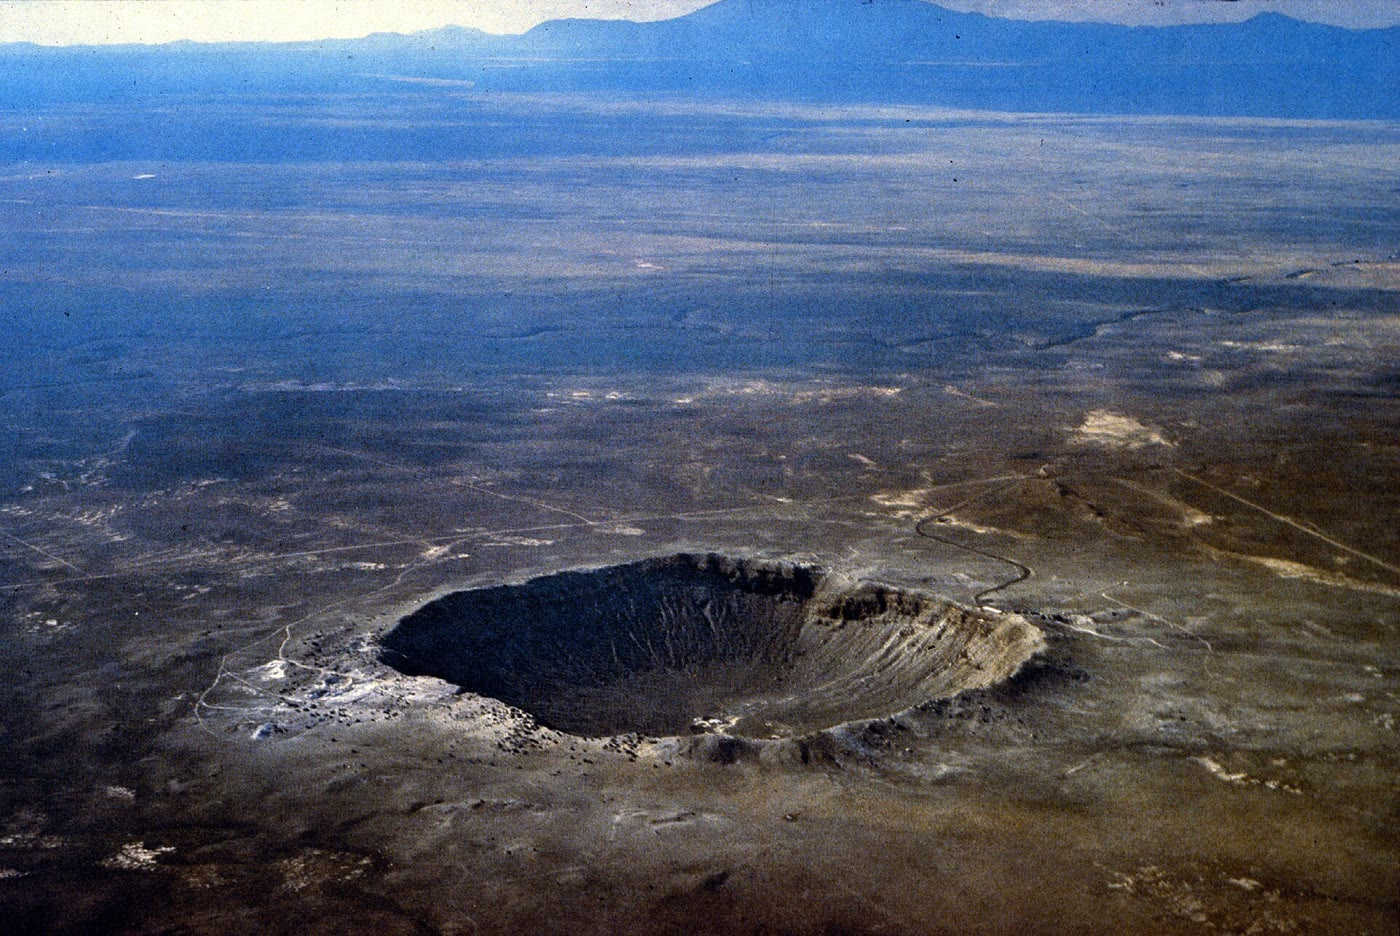
\includegraphics[width=0.66\linewidth]{images/book5/b3-barringer-crater.jpg}
\par\smallskip{\small Barringer Meteor Crater, Arizona, a \omterm{def:b3:planetary-interiors-surfaces:crater-morphology}{simple crater}
\qty{1.2}{km} across, formed about 50,000 years ago by an iron meteorite
some \qty{30}{m} across; the rim stands above the plateau and the \omterm{def:b3:planetary-interiors-surfaces:crater-morphology}{ejecta
blanket} spreads around it. Aerial photograph, USGS/D.~Roddy, public
domain.}\label{fig:b3:planetary-interiors-surfaces:barringer}
\end{omfigure}
% ledger: photo:b3-barringer, french:barringer

The excavation of a crater \qty{1}{km} across takes about six seconds, that
of a crater \qty{200}{km} across about a minute and a half. What size of
crater an impact makes depends on the projectile's energy, on gravity and
on the strength of the rock; the laws that relate them are fitted to
experiments and explosions in the form of products of dimensionless
groups, and are admitted here. Their spirit is in a balance of energies.
% ledger: french:transient

\begin{proposition}[Gravity-regime scaling]\label{prop:b3:planetary-interiors-surfaces:scaling}
If a fixed fraction of the impact energy $E$ lifts the excavated rock of
density $\rho$ against gravity $g$, the diameter of the crater grows as
\[
  D \propto \left(\frac{E}{\rho g}\right)^{1/4} .
\]
\end{proposition}

\begin{proof}
The excavated volume scales as $D^3$, its mass as $\rho D^3$, and it is
lifted by a height of order $D$: the work is of order $\rho g D^4$, which
is proportional to $E$.
\end{proof}

Part of the energy goes into heat, melting and the breaking of rock, so
the real laws fall between this one and simpler rules: a table often
quoted for the Earth takes a crater twenty times as wide as its stony
projectile. Gravity also sets where a crater stops being simple. The
walls of the transient bowl collapse when the weight of rock they hold,
of order $\rho g D/3$, exceeds the strength of the rock, so the
transition diameter varies as $1/g$: about \qty{4}{km} in crystalline
rock and \qty{2}{km} in sediments on the Earth, about \qty{20}{km} on the
Moon, where gravity is six times weaker.
% ledger: french:table21, french:transition, planet:Earth.gravity, planet:Moon.gravity

\section{Crater dating}\label{sec:b3:planetary-interiors-surfaces:dating}

A surface left alone collects craters at the rate at which bodies strike
it. Counting them dates the surface, provided the rate is known and the
craters are those of the surface, not of what lies beneath or of the
debris thrown from a neighbour.

\begin{definition}[Crater size--frequency distribution]\label{def:b3:planetary-interiors-surfaces:sfd}
The \emph{crater size--frequency distribution}\index{crater size--frequency distribution}
of a surface is the number $N(D)$ of craters of diameter at least $D$ per
unit area, as a function of $D$ (the cumulative distribution), or the
numbers counted in bins of diameter, usually each $\sqrt2$ times wider
than the last (the incremental distribution).
\end{definition}

\begin{definition}[Crater dating; production and chronology functions; equilibrium density]\label{def:b3:planetary-interiors-surfaces:crater-dating}
\emph{Crater dating}\index{crater dating} is the determination of the age
of a surface from the density of its craters. The \emph{crater production
function}\index{crater production function} is the shape of the
size--frequency distribution of the craters a surface acquires, $F(D) =
N(D)/N(\qty{1}{km})$, assumed the same at every age. The \emph{crater
chronology function}\index{crater chronology function} $N_1(T)$ is the
number of craters of \qty{1}{km} and more per unit area accumulated in a
time $T$. A surface is at the \emph{crater equilibrium
density}\index{crater equilibrium density} for craters of a given size
when each new crater erases, on average, as many old ones as it adds:
their number no longer grows.
\end{definition}

The model age of a surface follows from one count: $N(D)$ measured at any
$D$ gives $N_1 = N(D)/F(D)$, and $T$ solves $N_1(T) = N_1$. The lines
$N(D) = N_1(T)F(D)$ for fixed $T$ are called isochrons. For Mars, a widely
used production function is a polynomial of degree~11 in $\log_{10}D$, and
the chronology function has the form
\[
  N_1(T) = a\left(e^{bT} - 1\right) + cT , \qquad
  a = \qty{3.22e-14}{km^{-2}}, \ b = \qty{6.93}{Ga^{-1}}, \
  c = \qty{4.875e-4}{km^{-2}.Ga^{-1}} ,
\]
linear over the last three billion years, steeply exponential before. The
Moon's function has the same form with $a = \num{5.44e-14}$ and $c =
\num{8.38e-4}$. It was fitted to the ages of the Apollo and Luna landing
sites; that of Mars is the Moon's, scaled by an estimate of the ratio of
the cratering rates on Mars and on the Moon.
% ledger: craterstats:mars-pf, craterstats:mars-cf, craterstats:moon-cf, marchi:neukum

\begin{omfigure}
\centering
\begin{tikzpicture}
\begin{groupplot}[group style={group size=2 by 1, horizontal sep=1.6cm},
  width=0.48\linewidth, height=0.46\linewidth,
  tick label style={font=\scriptsize}, label style={font=\small}, title style={font=\small}]
\nextgroupplot[title={isochrons on Mars}, xmode=log, ymode=log, xmin=0.1, xmax=100,
  ymin=1e-8, ymax=100, xlabel={crater diameter $D$ (\unit{km})},
  ylabel={$N(D)$, craters $\geq D$ per \unit{km^2}},
  xtick={0.1,1,10,100}, xticklabels={0.1,1,10,100},
  ytick={1e-8,1e-6,1e-4,1e-2,1}]
\addplot[thick, black!50, dashed] table[x=D, y=eq] {figdata/out/bachelor-3-crater_sfd-iso.dat};
\addplot[omDef] table[x=D, y=N_0.1] {figdata/out/bachelor-3-crater_sfd-iso.dat};
\addplot[omDef] table[x=D, y=N_1] {figdata/out/bachelor-3-crater_sfd-iso.dat};
\addplot[omDef] table[x=D, y=N_3.5] {figdata/out/bachelor-3-crater_sfd-iso.dat};
\addplot[red!70!black, thick] table[x=D, y=N_4] {figdata/out/bachelor-3-crater_sfd-iso.dat};
\node[font=\tiny, omDef, anchor=north east] at (axis cs:0.75,8e-6) {0.1~Ga};
\node[font=\tiny, omDef, anchor=north east] at (axis cs:2.6,1e-5) {1~Ga};
\node[font=\tiny, omDef, anchor=north east] at (axis cs:9,3.5e-5) {3.5~Ga};
\node[font=\tiny, red!70!black, anchor=north east] at (axis cs:45,2.5e-5) {4~Ga};
\node[font=\tiny, black!60, anchor=south, rotate=-30] at (axis cs:25,3.5e-4) {equilibrium};
\nextgroupplot[title={chronology functions}, ymode=log, xmin=0, xmax=4.5,
  ymin=1e-5, ymax=0.3, xlabel={age $T$ (\unit{Ga})}, ylabel={$N_1$ per \unit{km^2}},
  legend style={font=\scriptsize, at={(0.03,0.97)}, anchor=north west}]
\addplot[thick, red!70!black] table[x=T, y=mars] {figdata/out/bachelor-3-crater_sfd-chron.dat};
\addlegendentry{Mars}
\addplot[thick, black!60, dashed] table[x=T, y=moon] {figdata/out/bachelor-3-crater_sfd-chron.dat};
\addlegendentry{Moon}
\end{groupplot}
\end{tikzpicture}
\par\smallskip{\small Left: isochrons of Mars, the cumulative densities of
craters on surfaces 0.1, 1, 3.5 and 4 billion years old, with the
equilibrium density (dashed), which caps every count: on a surface 4
billion years old the craters smaller than about \qty{0.7}{km} are at
equilibrium and no longer record the age. Right: the chronology functions
of Mars and of the Moon, the number of craters of \qty{1}{km} and more per
square kilometre against the age of the
surface.}\label{fig:b3:planetary-interiors-surfaces:sfd}
\end{omfigure}
% ledger: craterstats:mars-pf, craterstats:mars-cf, craterstats:moon-cf, craterstats:equilibrium

Craters are struck at random, independently of each other, so the number
$n$ found on an area is a Poisson variable.

\begin{proposition}[Counting error of a model age]\label{prop:b3:planetary-interiors-surfaces:poisson}
If $n$ craters are counted on an area $A$, the density $N = n/A$ has the
standard deviation $\sqrt n/A$, a relative error $1/\sqrt n$, and the model
age the standard deviation
\[
  \sigma_T = \frac{N_1(T)}{\sqrt n\,N_1'(T)} .
\]
\end{proposition}

\begin{proof}
A Poisson variable of mean $\lambda$ has variance $\lambda$, estimated by
$n$. The age is $T = N_1^{-1}(N_1)$; to first order $\sigma_T =
\sigma_{N_1}/N_1'(T)$, and $\sigma_{N_1} = N_1/\sqrt n$.
\end{proof}

The relative error of the count alone is ten percent for a hundred
craters. On a young surface, where $N_1$ is linear, the age inherits it:
$\sigma_T/T = 1/\sqrt n$. On an old one the steep function shrinks it, by
a factor of six at \qty{3.8}{Ga} (\cref{exo:b3:planetary-interiors-surfaces:11});
the model ages of old surfaces are then limited instead by the calibration
of the function itself. Two further limits bound a count. Small craters
saturate: on the oldest surfaces, craters below about \qty{0.7}{km} are at
the equilibrium density and stop recording time. And a surface may be renewed
without being erased: a lava flow that buries small craters but not the
rims of large ones leaves a distribution with a kink, old at large $D$ and
young at small $D$. The kink dates the \omterm{def:b3:planetary-interiors-surfaces:resurfacing}{resurfacing}.
% ledger: craterstats:equilibrium

\begin{definition}[Resurfacing]\label{def:b3:planetary-interiors-surfaces:resurfacing}
\emph{Resurfacing}\index{resurfacing} is the renewal of a planetary
surface, by lava, sediment, ice or deformation, that removes or buries its
craters and resets its crater clock.
\end{definition}

\section{Volcanism and tectonics beyond the Earth}\label{sec:b3:planetary-interiors-surfaces:volcanism}

Every terrestrial planet loses its internal heat through its lithosphere.
The Earth does it with moving plates; the others do it differently.

\begin{definition}[Stagnant lid]\label{def:b3:planetary-interiors-surfaces:stagnant-lid}
A planet has a \emph{stagnant lid}\index{stagnant lid} when its lithosphere
is a single rigid shell that does not take part in the convection of the
mantle below: heat crosses it by conduction and by the magma that rises
through it. On a mobile-lid planet like the Earth, the lithosphere is
broken into plates that sink back into the mantle.
\end{definition}

\begin{definition}[Heat-pipe volcanism]\label{def:b3:planetary-interiors-surfaces:heat-pipe}
\emph{Heat-pipe volcanism}\index{heat-pipe volcanism} is the loss of a
planet's internal heat mainly by magma rising through narrow conduits and
erupting at the surface, where the lavas cool and are buried by later
ones: the lithosphere is built from the top and carried downwards, cold.
\end{definition}

\begin{omfigure}
\centering
\begin{tikzpicture}[x=0.5cm, y=0.5cm, font=\scriptsize, >=stealth]
\foreach \dx/\name in {0/mobile lid, 9.5/stagnant lid, 19/heat pipe} {
  \begin{scope}[xshift=\dx*0.5cm]
  \fill[orange!15] (0,0) rectangle (8,4);
  \node[anchor=south] at (4,5.6) {\name};
  \end{scope}}
% mobile lid: plates, ridge, slab
\fill[omDef!35] (0,4) rectangle (3.9,4.8);
\fill[omDef!35] (4.1,4) rectangle (6.2,4.8);
\fill[omDef!35] (6.2,4.8) -- (7.6,1.6) -- (6.9,1.4) -- (5.5,4.0) -- cycle;
\fill[omDef!35] (6.55,4) rectangle (8,4.8);
\draw[->, thick] (3.6,5.1) -- (1.6,5.1); \draw[->, thick] (4.4,5.1) -- (6.0,5.1);
\draw[->, red!70!black] (4,1.0) -- (4,3.6);
\draw[black!60, ->] (2.0,3.4) arc (90:270:1.0 and 1.2);
\node[anchor=north] at (4,-0.2) {plates sink};
% stagnant lid
\begin{scope}[xshift=4.75cm]
\fill[omDef!35] (0,3.2) rectangle (8,4.8);
\draw[black!60, ->] (2.4,3.0) arc (90:270:1.2 and 1.2);
\draw[black!60, ->] (5.6,0.6) arc (-90:90:1.2 and 1.2);
\fill[red!70!black] (3.9,3.2) rectangle (4.1,4.8);
\fill[red!70!black] (3.0,4.8) -- (4,5.4) -- (5.0,4.8) -- cycle;
\node[anchor=north] at (4,-0.2) {one thick shell};
\end{scope}
% heat pipe
\begin{scope}[xshift=9.5cm]
\fill[omDef!35] (0,1.0) rectangle (8,4.8);
\foreach \x in {1.5,4,6.5} {\fill[red!70!black] (\x-0.1,1.0) rectangle (\x+0.1,4.8);
  \fill[red!70!black] (\x-0.6,4.8) -- (\x,5.2) -- (\x+0.6,4.8) -- cycle;}
\draw[->, thick] (2.75,4.3) -- (2.75,1.6); \draw[->, thick] (5.25,4.3) -- (5.25,1.6);
\node[anchor=north] at (4,-0.2) {lavas buried, lid cold};
\end{scope}
\end{tikzpicture}
\par\smallskip{\small Three ways of losing heat (schematic). Left: a
mobile lid, plates made at ridges and sinking at trenches, as on the
Earth. Centre: a \omterm{def:b3:planetary-interiors-surfaces:stagnant-lid}{stagnant lid}, one rigid shell over the convecting mantle,
crossed by the magma of a few long-lived volcanoes. Right: heat pipes,
magma rising through a thick cold lithosphere in narrow conduits, its lavas
buried by later ones and carried
down.}\label{fig:b3:planetary-interiors-surfaces:lids}
\end{omfigure}

Mars has a \omterm{def:b3:planetary-interiors-surfaces:stagnant-lid}{stagnant lid}. Without plates to carry them away from their
sources, its volcanoes grew in place for a long time over the Tharsis
bulge. Olympus Mons, the largest known volcano in the Solar System, stands
\qty{27}{km} high on a base more than \qty{600}{km} across, ringed by a
scarp up to \qty{6}{km} high; the three Tharsis Montes nearby are each 350
to \qty{400}{km} across. A load so large bends the lithosphere, and the
width of the moat it digs measures, as on the Earth, the elastic thickness
of the lid.
% ledger: nasa:olympus-mons

\begin{omfigure}
\centering
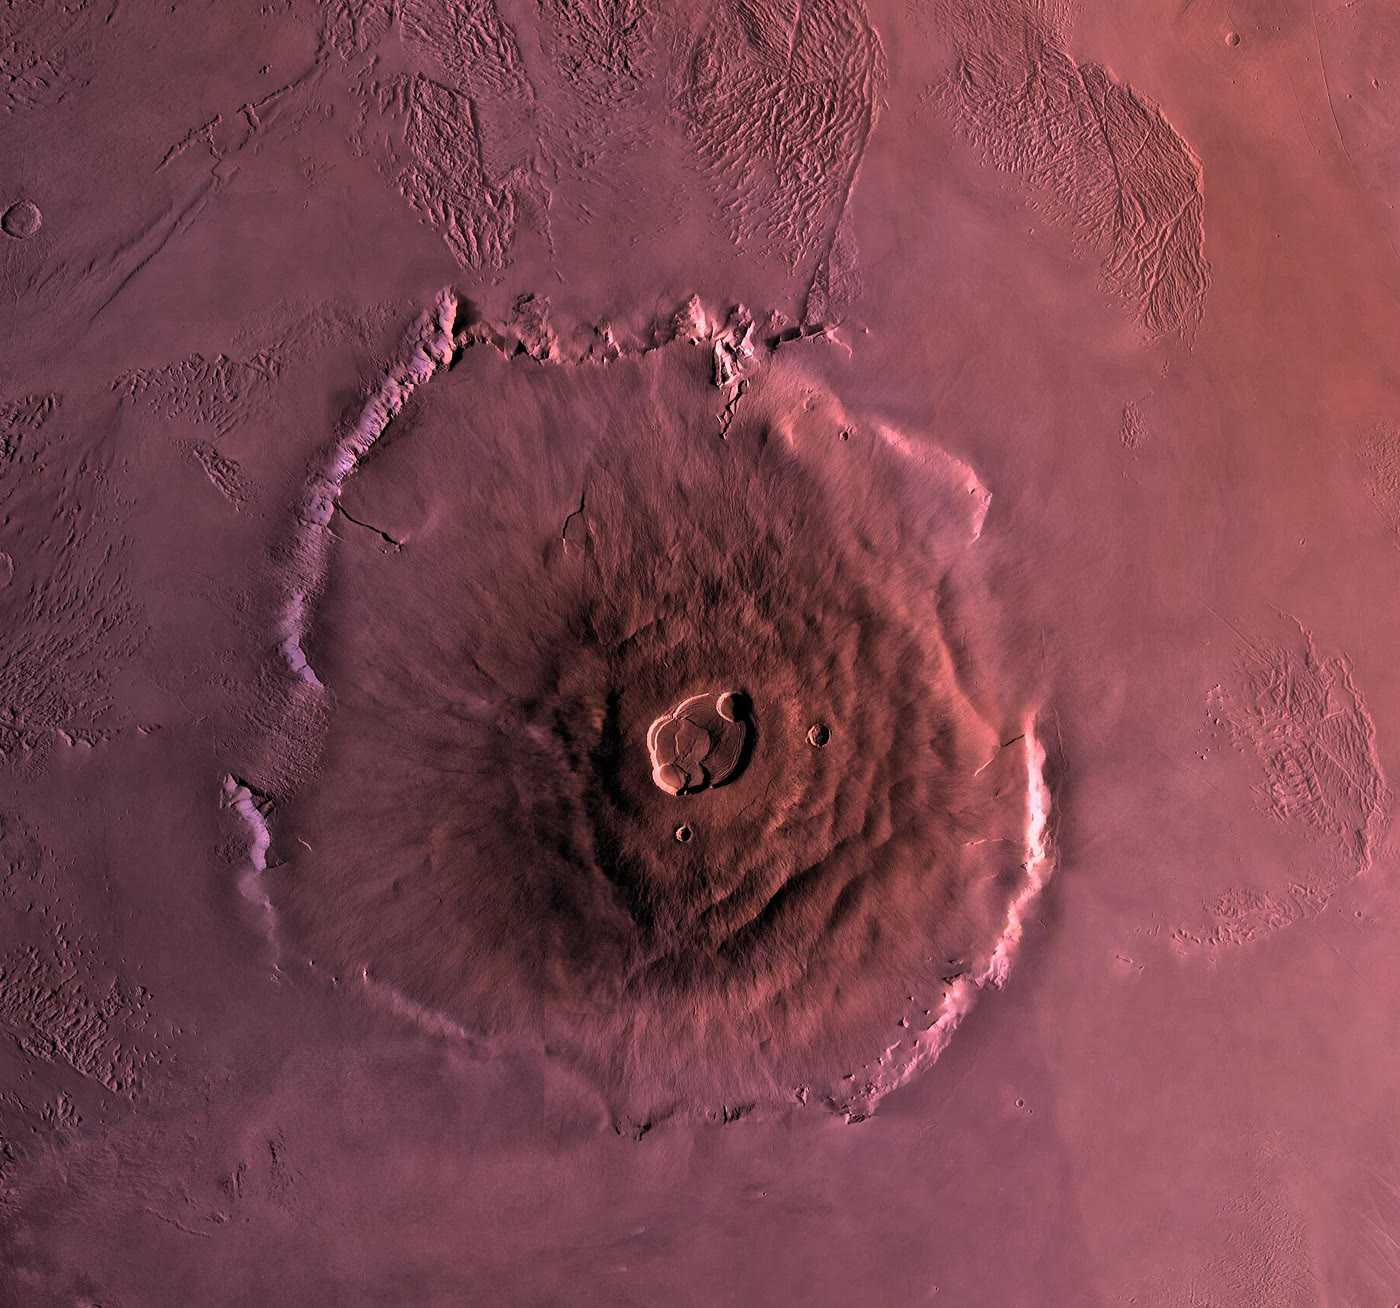
\includegraphics[width=0.48\linewidth]{images/book5/b3-olympus-mons.jpg}
\par\smallskip{\small Olympus Mons on Mars, a mosaic of images of the
Viking orbiters: the summit calderas at the centre, the flanks of lava
flows and the cliffed scarp that rings the base, some \qty{600}{km} across.
NASA/JPL/USGS, public domain.}\label{fig:b3:planetary-interiors-surfaces:olympus}
\end{omfigure}
% ledger: photo:b3-olympus-mons, nasa:olympus-mons

Venus, the Earth's twin in size, has by far the fewest impact craters of
any rocky planet except the Earth. Its surface features may be on average
as young as 150 million years, with older patches between them:
volcanism and deformation renewed most of its surface, perhaps piecemeal
over a long time, perhaps faster. Venus has thousands of volcanoes and no
sign of moving plates.
% ledger: nasa:venus-surface, planet:Venus.diameter, planet:Earth.diameter

Io, the innermost large moon of Jupiter, loses more than
\qty{2.5}{W.m^{-2}} through its surface, some 27 times the Earth's average
of \qty{0.092}{W.m^{-2}}. Its heat is not that of radioactivity: it is
made by the tides.
% ledger: veeder:io-heat, dd10:split

\begin{definition}[Tidal heating]\label{def:b3:planetary-interiors-surfaces:tidal-heating}
\emph{Tidal heating}\index{tidal heating} is the heat produced inside a
body by the friction of the deformation that a varying tide imposes on it.
A moon in synchronous rotation on an eccentric orbit sees the tide of its
planet change in strength and swing back and forth during each orbit.
\end{definition}

\begin{proposition}[Tidal power of a synchronous moon]\label{prop:b3:planetary-interiors-surfaces:tidal-power}
A moon of radius $R$ in synchronous rotation, on an orbit of mean motion
$n$ and small eccentricity $e$, dissipates the power
\[
  \dot E = \frac{21}{2}\,\frac{k_2}{Q}\,\frac{(nR)^5}{G}\,e^2 ,
\]
where $Q$ is the moon's tidal quality factor, so that $k_2/Q$ measures
the part of the tidal deformation lost as heat.
\end{proposition}

The proposition is admitted. Tides that dissipate energy also round off
an orbit; Io's stays elliptical, of eccentricity 0.004, because the
precisely timed pulls of Europa and Ganymede perturb it, their orbital
periods of 1.77, 3.55 and \qty{7.15}{days} standing almost exactly as
1:2:4 (\cref{exo:b3:planetary-interiors-surfaces:8}). Its surface rises
and falls by as much as \qty{100}{m} at each orbit. The volcanoes
cover Io with lava faster than craters can form on it; one model of
how its heat escapes is \omterm{def:b3:planetary-interiors-surfaces:heat-pipe}{heat-pipe volcanism}, which would keep a thick,
cold lithosphere under its fiery surface.
% ledger: nasa:galilean-orbits, beuthe:tidal-power, nasa:io-orbit, nasa:io-facts

\begin{definition}[Subsurface ocean]\label{def:b3:planetary-interiors-surfaces:ocean-world}
A \emph{subsurface ocean}\index{subsurface ocean} is a global layer of
liquid water under the ice shell of a moon or dwarf planet, kept liquid by
tidal and radiogenic heat.
\end{definition}

\begin{definition}[Cryovolcanism]\label{def:b3:planetary-interiors-surfaces:cryovolcanism}
\emph{Cryovolcanism}\index{cryovolcanism} is the eruption of water, brines
or other volatile liquids and vapours, instead of molten rock, onto the
icy surface of a moon or dwarf planet.
\end{definition}

Europa's ice shell, measured by the microwave radiometer of the Juno
spacecraft in the region it flew over, averages about \qty{29}{km} thick;
beneath it lies a salty ocean holding twice as much water as all the
Earth's oceans. On Saturn's moon Enceladus, only about \qty{500}{km}
across, the Cassini spacecraft found in 2005 jets of ice grains and gas
leaving warm fractures near the south pole at about
\qty{400}{m.s^{-1}}. Its gravity and the wobble of its rotation showed
that the jets draw on a global ocean, under an ice shell 20 to
\qty{25}{km} thick on average and perhaps only 1 to \qty{5}{km} at the
south pole.
% ledger: jpl:europa-shell, nasa:europa-ocean, nasa:enceladus

\section{Large cores and small ones}\label{sec:b3:planetary-interiors-surfaces:cores}

The four measured cores make an odd family. Relative to its radius, the
Earth's core reaches 0.55 of the way to the surface and Mars's 0.54; the
Moon's 0.19; Mercury's 0.82. Differentiation, in the Year~2 volume, sorts
metal from silicate inside each body, but cannot make the proportions of
metal so different. Giant impacts can. The Moon is thought to have formed
from the debris of a collision between a body the size of Mars and the
young Earth about 4.5 billion years ago, the metal of the impactor joining
the Earth's core and the Moon gathering mostly mantle rock, hence its
small core. Similar impacts may have stripped a large part of the silicate
mantle of Mercury and left it the iron-rich planet whose core fills most
of it. The cores record, as the craters do, a history of collisions.
% ledger: data:prem, jpl:insight-interior, nasa:moon-core, agu:mercury-core, french:giant-impacts

\section{Exercises}

\begin{exercise}[$\star$]\label{exo:b3:planetary-interiors-surfaces:1}
Mercury has a mean density of \qty{5429}{kg.m^{-3}}, a moment-of-inertia
factor of 0.35 and a radius of \qty{2440}{km}. With a two-layer model and a
mantle of \qty{3300}{kg.m^{-3}}, compute the relative radius of the core,
its radius in kilometres and its density.
\end{exercise}

\begin{exercise}[$\star$]\label{exo:b3:planetary-interiors-surfaces:2}
A stony projectile \qty{50}{m} across, of density \qty{3500}{kg.m^{-3}},
strikes the Earth vertically at \qty{20}{km.s^{-1}}. Compute its mass and
its kinetic energy, in joules and in megatons of explosive
($\qty{1}{Mt} = \qty{4.2e15}{J}$). What diameter of crater does the rule
of twenty projectile diameters give?
\end{exercise}

\begin{exercise}[$\star$]\label{exo:b3:planetary-interiors-surfaces:3}
On a Martian plain of \qty{100000}{km^2}, 120 craters of \qty{1}{km} and
more are counted. Compute $N_1$, its relative error, and the model age of
the plain with its error.
\end{exercise}

\begin{exercise}[$\star$]\label{exo:b3:planetary-interiors-surfaces:4}
Io, of radius \qty{1821.5}{km}, loses \qty{2.5}{W.m^{-2}}. Compute its
total heat loss and compare it with the Earth's, \qty{47}{TW}, in total and
per square metre (\qty{0.092}{W.m^{-2}}).
\end{exercise}

\begin{exercise}[$\star\star$]\label{exo:b3:planetary-interiors-surfaces:5}
Mars has a mass of \qty{6.417e23}{kg} and a radius of \qty{3389.5}{km}.
(a)~Compute its mean density, its surface gravity and $\rho gR$.
(b)~Treating it as a uniform incompressible sphere of rigidity
\qty{67}{GPa}, compute its \omterm{def:b3:planetary-interiors-surfaces:love-number}{Love number} $k_2$. (c)~The measured value is
$0.153 \pm 0.017$. What does the comparison say?
\end{exercise}

\begin{exercise}[$\star\star$]\label{exo:b3:planetary-interiors-surfaces:6}
On the Earth ($g = \qty{9.8}{m.s^{-2}}$) the simple-to-complex transition
occurs at about \qty{4}{km} in crystalline rock and \qty{2}{km} in
sediments. (a)~Assuming that the transition diameter varies as $1/g$,
predict it on the Moon ($g = \qty{1.62}{m.s^{-2}}$) and on Mars and
Mercury ($g = \qty{3.7}{m.s^{-2}}$); compare with the \qty{20}{km}
observed on the Moon. (b)~If collapse begins when $\rho gD/3$ exceeds the
strength $Y$ of the rock, what strength does the Earth's crystalline
transition give, for $\rho = \qty{2600}{kg.m^{-3}}$?
\end{exercise}

\begin{exercise}[$\star\star$]\label{exo:b3:planetary-interiors-surfaces:7}
A surface carries $\num{2.0e-3}$ craters of \qty{1}{km} and more per
square kilometre. Find its model age with the chronology function of Mars,
by solving the equation numerically. What age would the lunar function have
given, and why may the two not be exchanged?
\end{exercise}

\begin{exercise}[$\star\star$]\label{exo:b3:planetary-interiors-surfaces:8}
The orbital periods of Io, Europa and Ganymede are 1.769138, 3.551181 and
\qty{7.154553}{days}. (a)~Compute the ratios of successive periods.
(b)~Compute $1/P_I - 3/P_E + 2/P_G$ and comment. (c)~Why can resonances
keep an eccentricity that tides would otherwise remove?
\end{exercise}

\begin{exercise}[$\star\star$]\label{exo:b3:planetary-interiors-surfaces:9}
Io orbits Jupiter in \qty{1.769138}{days} with eccentricity 0.004.
Compute the power the tidal-power proposition gives per unit of $k_2/Q$,
and the value of $k_2/Q$ that would supply Io's heat loss of
\cref{exo:b3:planetary-interiors-surfaces:4}.
\end{exercise}

\begin{exercise}[$\star\star\star$]\label{exo:b3:planetary-interiors-surfaces:10}
For the Moon, $\bar\rho = \qty{3340}{kg.m^{-3}}$ and $C = 0.394$.
(a)~Show that in the two-layer model $\mathrm dx^2/\mathrm dC =
\tfrac52\bar\rho/(\bar\rho - \rho_m)$ at fixed $\rho_m$. (b)~With the
mantle density that gives a core of $x = 0.19$, \qty{3288}{kg.m^{-3}},
what are $x$ and $\rho_c$ when $C = 0.395$, and when $C = 0.393$?
(c)~What does this say about weighing a small core with the moment of
inertia?
\end{exercise}

\begin{exercise}[$\star\star\star$]\label{exo:b3:planetary-interiors-surfaces:11}
(a)~For 100 craters, compute the counting error of the model age of a
Martian surface \qty{1.0}{Ga} old and of one \qty{3.8}{Ga} old.
(b)~Show that on the linear part of the chronology function $\sigma_T/T =
1/\sqrt n$. (c)~Why are the ages of old surfaces then still uncertain?
\end{exercise}

\begin{exercise}[$\star\star\star$]\label{exo:b3:planetary-interiors-surfaces:12}
Europa, of radius \qty{1560.8}{km}, orbits in \qty{3.551181}{days} with
eccentricity 0.009. (a)~If Europa dissipated tides with the same $k_2/Q$
as Io, what fraction of Io's tidal power would it make, and what heat flow?
(b)~Why is the assumption doubtful for a moon with an ocean under its ice?
\end{exercise}

\section{Problem: Two Plains on Mars}

\begin{problem}[{Weekend problem --- the core of Mars and the ages of two
invented lava plains}]
\label{pb:b3:planetary-interiors-surfaces:1}
Mars has a mass of \qty{6.4169e23}{kg}, a radius of \qty{3389.5}{km} and a
moment-of-inertia factor of 0.366. Two invented plains, A and B, lie on its
volcanic provinces; their craters have been counted on images in bins
$\sqrt2$ wide.

\medskip\noindent\textbf{Part I --- The core.}
\begin{enumerate}
\item Compute the mean density of Mars.
\item With a two-layer model and a mantle of \qty{3500}{kg.m^{-3}}, compute
  the relative radius of the core, its radius in kilometres and its
  density.
\item InSight measured a core radius of \qty{1830}{km}. What mantle and core
  densities does the two-layer model then require?
\item Compare that core density with the density of the Earth's outer core
  just below its top, \qty{9900}{kg.m^{-3}} in the reference Earth model,
  and say why a lower value is expected for Mars, and what else it
  suggests.
\item The uniform-sphere \omterm{def:b3:planetary-interiors-surfaces:love-number}{Love number} of Mars with a rigidity of
  \qty{67}{GPa} is 0.109; the measured one is 0.153. Which observation came
  first, and what did it already say about the core?
\item The crust of Mars is 20 to \qty{37}{km} thick. What fraction of the
  planet's volume does it hold? Was it right to ignore it?
\end{enumerate}

\medskip\noindent\textbf{Part II --- The counts on plain A.} Plain A
covers \qty{80000}{km^2}. Its craters, by bin of diameter (km):
\begin{center}
\small
\begin{tabular}{lccccccccc}
\hline
bin & 1--1.41 & 1.41--2 & 2--2.83 & 2.83--4 & 4--5.66 & 5.66--8 & 8--11.3 & 11.3--16 & 16--22.6 \\
\hline
plain A & 38 & 6 & 5 & 3 & 0 & 0 & 0 & 1 & 1 \\
plain B & 48 & 8 & 31 & 12 & 7 & 2 & 0 & 2 & 2 \\
\hline
\end{tabular}
\end{center}
\begin{enumerate}[resume]
\item Compute the cumulative counts of plain A, from \qty{1}{km} up.
\item Compute $N(\qty{1}{km})$ per square kilometre and its standard
  deviation.
\item The production function gives $F(\qty{2}{km}) = 0.147$ and
  $F(\qty{1.41}{km}) = 0.355$. Are the counts at 1.41 and \qty{2}{km}
  consistent with the shape of the production function?
\item Is plain A anywhere near the equilibrium density,
  \qty{0.072}{km^{-2}} at \qty{1}{km}?
\item Why are the bins chosen $\sqrt2$ wide?
\item Clusters and chains of small craters are left out of a count. Why?
\end{enumerate}

\medskip\noindent\textbf{Part III --- Model ages.} Use the chronology
function of Mars.
\begin{enumerate}[resume]
\item Compute the model age of plain A. Check that the exponential term
  may be neglected.
\item Compute its counting error.
\item What age would the lunar chronology have given?
\item Plain B covers \qty{120000}{km^2}. Using its craters of \qty{2}{km}
  and more, compute $N(\qty{2}{km})$, then $N_1$, then its model age, by
  solving the equation numerically.
\item Compute the counting error of that age.
\item Compare the relative errors of the two ages and explain the
  difference.
\end{enumerate}

\medskip\noindent\textbf{Part IV --- The buried craters of plain B.}
\begin{enumerate}[resume]
\item How many craters between 1 and \qty{2}{km} should plain B carry if
  its whole surface had the age of question~16? How many does it carry?
\item Assume that lava buried every crater smaller than \qty{2}{km} at a
  time $T_r$ and spared the larger ones. Compute $T_r$ from the
  \qty{1}{}--\qty{2}{km} craters.
\item Compute the counting error of $T_r$.
\item Take a fresh \omterm{def:b3:planetary-interiors-surfaces:crater-morphology}{simple crater} on Mars to be a fifth as deep as it is
  wide (an assumption of this problem). How thick must the lava be to bury
  a \qty{2}{km} crater, and why do the larger ones still show?
\item Could the lava of plain B and that of plain A belong to one episode
  of volcanism?
\item Give the model age of plain A, in billions of years, to two
  significant figures.
\end{enumerate}
\end{problem}
% ledger: nasa:mars, jpl:insight-interior, yoder:mars-k2, data:prem, craterstats:mars-pf, craterstats:mars-cf, craterstats:moon-cf, craterstats:equilibrium
